
\newpage
\chapter{Cadre générale du projet}
\addcontentsline{toc}{section}{\textbf{Chapitre 1 : Cadre général du projet}}
 \fontsize{12pt}{12pt}\selectfont

 \addcontentsline{toc}{section}{Introduction}
 Ce chapitre a pour objectif de présenter le cadre général de notre projet de fin d'année. Il s'articulera autour 
 de l'étude et de l'analyse critique de l'existant, permettant de mieux situer notre travail. Nous y exposerons 
 ensuite la problématique abordée, les objectifs visés, ainsi que les tâches à réaliser, avant de conclure par la 
 méthodologie adoptée pour mener à bien ce projet.
 \section{Contexte de travail}
 C'est dans le cadre de notre deuxième projet de fin d'année au sein de l'Ecole Nationale Supérieure 
 d'Ingénieurs de Tunis (ENSIT), que nous proposons la conception et l'implémentation d'une application 
 intelligente de pépinière intégrant une plateforme e-commerce dédiée à la commercialisation des plantes, 
 ainsi qu'un système de diagnostic basé sur l'intelligence artificielle. Cette application permet aux 
 utilisateurs de capturer des images de leurs plantes, d'analyser leur état de santé à l'aide de techniques 
 de vision par ordinateur et de recevoir des recommandations adaptées. L'objectif est de fournir une solution 
 numérique innovante facilitant à la fois la gestion des pépinières et l'assistance aux utilisateurs dans l'entretien 
 et le suivi de leurs plantes.
\section{Etude de l'existant}
Afin de mieux comprendre les solutions disponibles dans ce domaine et didentifier les fonctionnalités les 
plus pertinentes, nous avons jugé nécessaire d'analyser quelques applications existantes. Les exemples 
retenus pour cette étude sont : PictureThis, Pl@ntNet et Bloomscape.

\subsection{Bloomscape}
\textbf{Bloomscape} est une plateforme de vente en ligne spécialisée dans la commercialisation de plantes et 
d'accessoires de jardinage. Elle permet aux clients d'acheter des plantes d'intérieur, des pots, des outils 
et des produits d'entretien. Cependant, elle ne propose aucun module de diagnostic ou d'analyse de l'état de 
santé des plantes à partir d'images, et n'intègre pas de fonctionnalités intelligentes permettant d'orienter 
l'utilisateur dans le traitement des plantes \cite{BloomscapeRef}.

La \autoref{fig:bloomscape} est une capture d'écran de Bloomscape.

\begin{figure}[H]
\centering
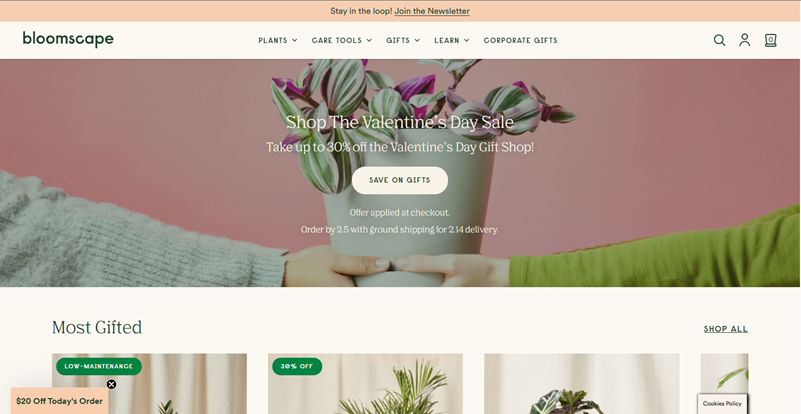
\includegraphics[width=0.6\textheight]{images/bloomscape.png}
\caption{ Capture d'écran de la page accueil de BloomscapeRef1 \cite{BloomscapeRef1}.}
\label{fig:bloomscape}
\end{figure}

\subsection{PictureThis}
\textbf{PictureThis} est une application mobile dédiée à l'identification des plantes à partir d'images. 
Elle permet aux utilisateurs de reconnaître rapidement une espèce végétale en prenant une photo, puis fournit 
un diagnostic automatique des maladies ainsi que des conseils de soins adaptés. Cette solution s'adresse 
principalement aux amateurs de jardinage souhaitant obtenir des informations sur l'état de leurs plantes. 
Toutefois, elle ne propose aucune fonctionnalité de vente \cite{pictureThisRef}.

La \autoref{fig:picturethis} présente la page d'accueil de l'application PictureThis.
\begin{figure}[H] 
\centering
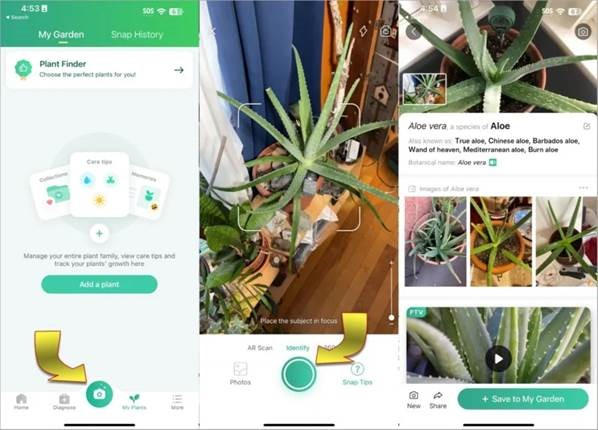
\includegraphics[height=0.3
\textheight]{images/picturethis.jpg}
\caption{ Page d'accueil de PictureThis \cite{pictureThisRef1}.}
\label{fig:picturethis}
\end{figure}
\subsection{Pl@ntNet}
\textbf{Pl@ntNet} est une application gratuite permettant l'identification des espèces végétales à partir 
d'images, s'appuyant sur une base de données enrichie par les contributions des utilisateurs. Bien que cette 
solution soit fiable sur le plan scientifique, elle reste principalement orientée vers l'identification des 
plantes et ne propose ni diagnostic approfondi des maladies ni fonctionnalités de vente ou de gestion de produits \cite{plantNetRef1}.

La \autoref{fig:plantnet} montre la page d'accueil de Pl@ntNet.
\begin{figure}[H]
\centering
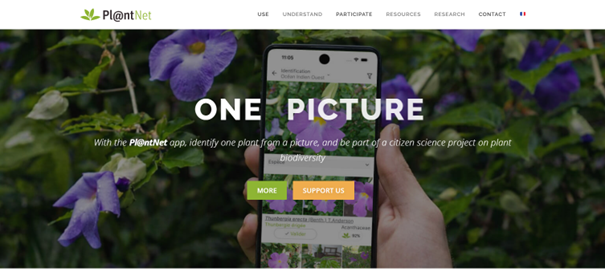
\includegraphics[width=0.5\textheight]{images/plantnet.png}
\caption{  Capture d'écran de la page accueil de Pl@ntNet \cite{plantNetRef1}.}
\label{fig:plantnet}
\end{figure}

\section{Critique de l'existant}
Certaines applications telles que PictureThis et Pl@ntNet permettent de reconnaitre les plantes, mais elles 
restent limitées en matière de vente en ligne et ne sont pas destinées aux pépinières. De plus, Pl@ntNet ne 
propose ni diagnostic des maladies ni recommandations de traitement. En revanche, Bloomscape est spécialisée 
dans la vente de plantes, mais elle n'intègre aucune fonctionnalité de diagnostic ni de recommandation intelligente 
pour le soin des plantes. Ainsi, aucune de ces solutions ne répond simultanément à l'ensemble des besoins : 
Identification des plantes, Diagnostic des plantes, Recommandation de traitements, Vente en ligne, Cible pépinières.
\newline
Le tableau \ref{tab:comparatif} représente les résultats de l'étude comparative réalisée.
\begin{table}[H]
\centering
\caption{Comparaison des fonctionnalités des applications}
\label{tab:comparatif}
\begin{tabular}{|l|c|c|c|}
\hline
\textbf{Critères} & \textbf{PictureThis} & \textbf{Pl@ntNet} & \textbf{Bloomscape} \\
\hline
Identification des plantes & Oui & Oui & Non \\
Diagnostic des plantes & Oui & Non & Non \\
Recommandation de traitements & Oui & Non & Non \\
Vente en ligne & Non & Non & Oui \\
Cible pépinières & Non & Non & Non \\
Payant & Oui & Non & Oui \\
\hline
\end{tabular}
\end{table}
\section{Problématique}
Après une analyse de la situation actuelle, nous avons constaté qu'une part 
importante du temps est consacrée à la gestion manuelle des activités liées aux 
pépinières, ainsi qu'à l'identification souvent approximative de l'état de santé 
des plantes. L'absence d'une application numérique unifiée intégrant à la fois des
 services de commercialisation des plantes et un système de diagnostic intelligent
  complique la gestion des pépinières et le suivi de l'état de santé des plantes, 
  ce qui peut conduire à des décisions peu adaptées en matière de traitement, 
  d'entretien et d'achat.
\section{Objectifs du projet}
Dans le but de répondre aux attentes des utilisateurs et d'intégrer une approche 
innovante dans le domaine de la pépinière, ce projet vise à atteindre les 
objectifs suivants :
\begin{enumerate}
\item Mettre en place une plateforme e-commerce permettant l'achat en ligne de 
plantes de manière simple, rapide et sécurisée.
\item Offrir aux utilisateurs un accès clair et structuré aux informations 
essentielles relatives aux plantes proposées à la vente.
\item Intégrer un système intelligent capable d'analyser les symptômes observés 
sur les plantes afin d'identifier les maladies, carences ou anomalies possibles.
\item Proposer des recommandations adaptées basées sur le diagnostic effectué, 
incluant des solutions de traitement et des conseils d'entretien.
\item Faciliter la prise de décision des utilisateurs en combinant vente de 
plantes et assistance intelligente au sein d'une seule plateforme.
\item Améliorer l'expérience utilisateur en fournissant une interface intuitive 
et des résultats compréhensibles, même pour les utilisateurs non experts.
\end{enumerate}
\section{Travail demandé}
Le travail demandé dans le cadre de ce projet consiste à analyser, concevoir et 
implémenter une solution applicative complète dédiée à la gestion d'une pépinière 
en ligne. Cette solution s'articule autour de deux axes principaux : une plateforme 
e-commerce pour la vente des plantes et un système intelligent pour le diagnostic et la 
recommandation. Les fonctionnalités de base associées à cette solution sont détaillées dans la suite :
\begin{itemize}
 \renewcommand{\labelitemi}{•}
\item \textbf{Inscription et authentification:} L'utilisateur doit remplir un formulaire 
d'inscription comprenant ses informations personnelles ainsi qu'un e-mail valide et un mot 
de passe pour l'authentification.
\newline Ces données permettront la gestion sécurisée de son compte, l'accès à l'historique 
des commandes et l'utilisation du système intelligent.
\item \textbf{Gestion du catalogue et des achats:} La plateforme permet à l'utilisateur de 
consulter les plantes disponibles, d'accéder à leurs fiches descriptives, de passer des 
commandes et de suivre l'état de ses achats. Un panier interactif et un système de paiement 
sécurisé sont intégrés afin de garantir une expérience fluide.
\item \textbf{Diagnostic intelligent des plantes:} L'utilisateur peut charger une photo qui 
sera analysée grâce aux modèles d'IA implémentés afin de proposer un diagnostic préliminaire 
sur l'état de la plante.
\item \textbf{Recommandations personnalisées:} À la suite du diagnostic, la plateforme fournit 
des recommandations adaptées concernant les traitements, l'entretien et les conditions optimales 
de croissance. Ces recommandations visent à améliorer la santé et la durabilité des plantes.
\end{itemize}
\section{Méthodologie de travail}
Dans le cadre de ce projet combinant une plateforme e-commerce et un système intelligent de 
diagnostic et de recommandation, nous avons opté pour deux méthodologies complémentaires : le 
\textbf{modèle en V} pour le développement de la plateforme applicative et \textbf{CRISP-DM} pour 
la conception du système intelligent.

Le choix du modèle en V se justifie par la nécessité d'adopter une démarche structurée et rigoureuse 
dans la conception et la réalisation de la plateforme e-commerce. En effet, ce modèle repose sur une 
correspondance entre les phases de spécification et les phases de validation, permettant ainsi d'assurer 
la qualité et la fiabilité du système développé \cite{vModelRef}.

et la \autoref{cycleV1} présente les étapes du cycle en V.

\begin{figure}[H] 
\centering
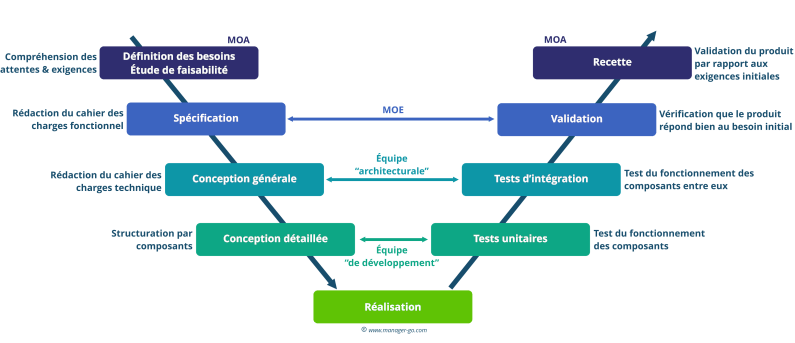
\includegraphics[width=0.5\textheight]{images/CycleV.png}
\caption{Le cycle en V \cite{cycleV}.}
\label{fig:cycleV1}
\end{figure}

La méthodologie CRISP-DM a été retenue pour encadrer la conception du système intelligent de diagnostic 
et de recommandation. Elle propose une démarche structurée en plusieurs étapes allant de la compréhension 
du métier à l'évaluation du modèle, facilitant ainsi l'exploitation des données et la mise en œuvre de solutions 
d'analyse pertinentes \cite{crispdmRef}.

La \autoref{fig:crispDM} illustre les différentes étapes de la méthodologie CRISP-DM.

\begin{figure}[ht]
\centering
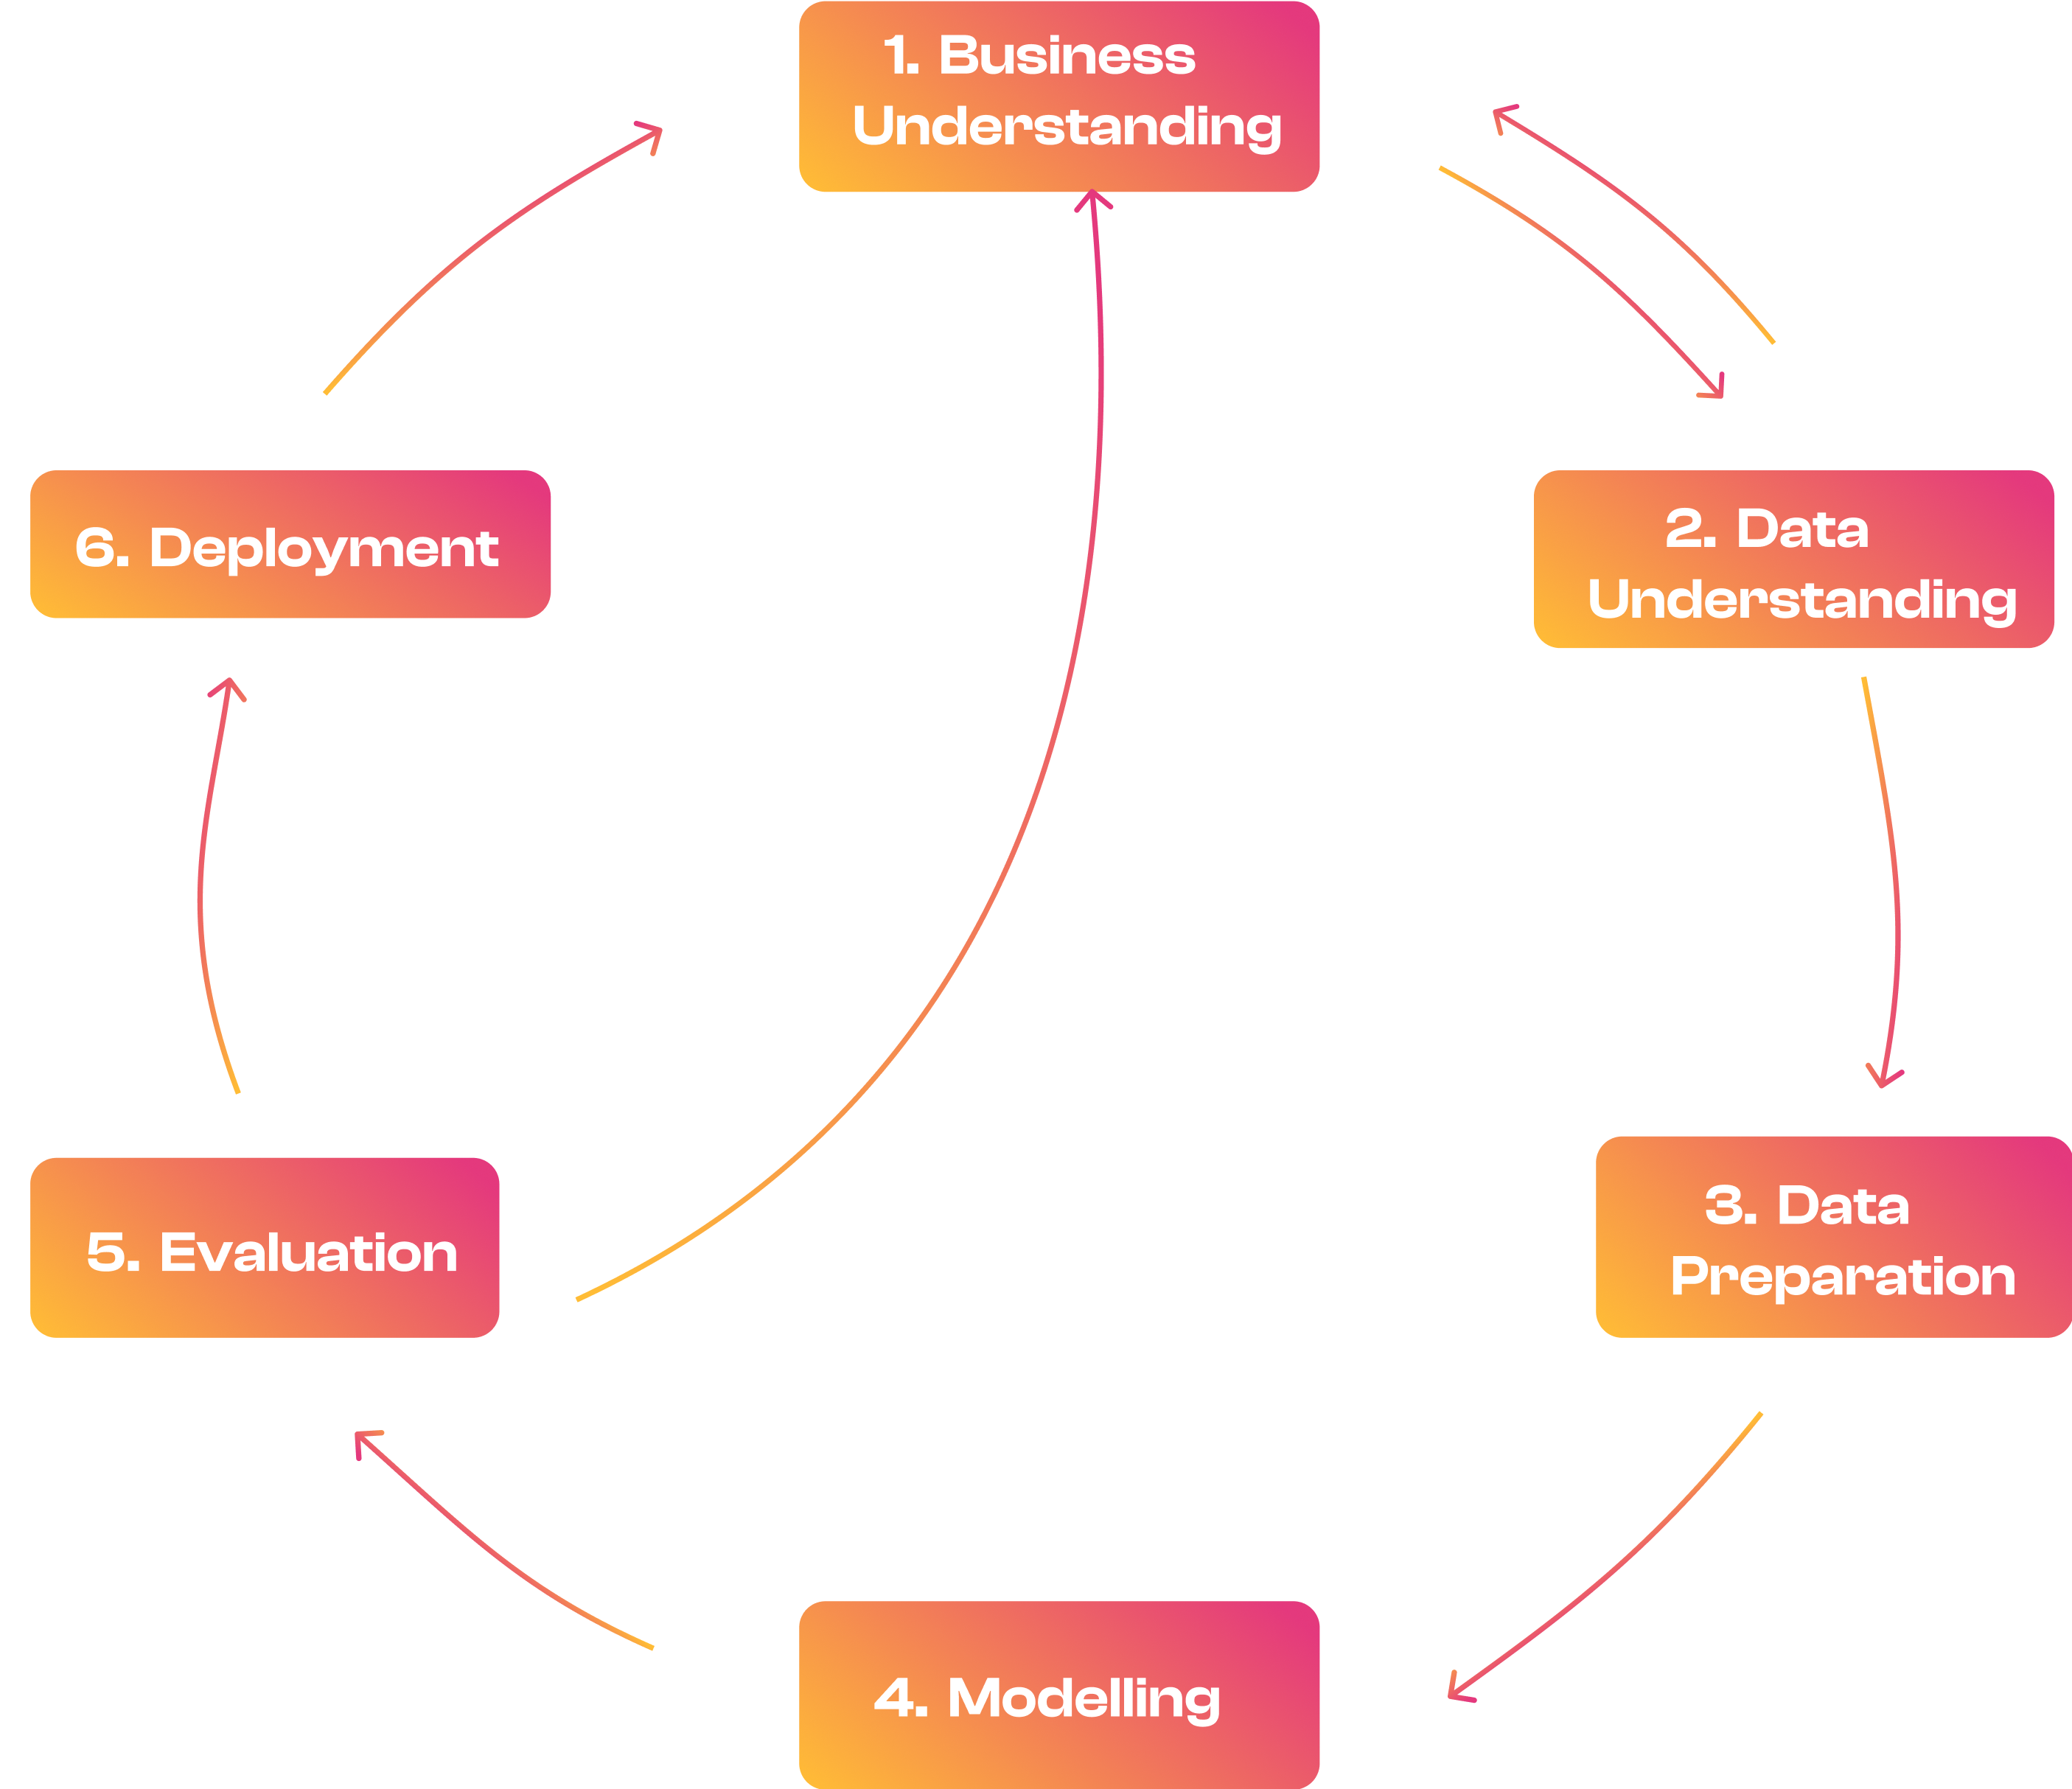
\includegraphics[width=0.4\textheight]{images/crispdm.png}
\caption{Les étapes de la méthodologie CRISP-DM \cite{crispDM1}.}
\label{fig:crispDM}
\end{figure}

L'association du modèle en V et de CRISP-DM permet ainsi de concilier rigueur et structuration. Le modèle 
en V assure une organisation claire du développement applicatif et des phases de validation, tandis que 
CRISP-DM garantit une approche méthodique dans la conception du système intelligent. Cette combinaison 
constitue un choix adapté aux objectifs et aux contraintes de notre projet.




\section*{Conclusion}
\addcontentsline{toc}{section}{Conclusion}
Dans ce chapitre introductif, nous avons présenté le contexte général et le sujet de notre projet. 
Nous y avons également défini la problématique, précisé les objectifs visés ainsi que le travail 
demandé. Le chapitre suivant sera consacré à l'analyse et à la spécification des besoins du système à développer.